\documentclass[11pt, letterpaper]{article}
\usepackage[margin=1in]{geometry}
\usepackage{enumitem}
\usepackage{parskip}
\usepackage{titlesec}
\usepackage{booktabs}
\usepackage{tabularx}
\usepackage{graphicx}
\usepackage{pgfgantt}
\usepackage{tikz}
\usetikzlibrary{arrows.meta, positioning}
\usepackage[hidelinks]{hyperref}

% Section formatting
\titleformat{\section}{\normalfont\large\bfseries}{\thesection}{1em}{}[\titlerule]
\titleformat{\subsection}{\normalfont\normalsize\bfseries}{\thesubsection}{1em}{}
\titleformat{\subsubsection}{\normalfont\normalsize\itshape}{\thesubsubsection}{1em}{}
\titlespacing{\section}{0pt}{12pt}{6pt}
\titlespacing{\subsection}{0pt}{8pt}{4pt}
\titlespacing{\subsubsection}{0pt}{6pt}{2pt}

\begin{document}

% ─── Title Page ──────────────────────────────────────────────────────────────
\begin{titlepage}
    \centering
    \vspace*{2cm}
    {\large University of Pennsylvania}\\[0.5em]
    {\large CIS 5680: Game Design Practicum}\\[3cm]
    {\LARGE \textbf{Game Design Document}}\\[1em]
    {\Huge \textbf{Umbra}}\\[0.5em]
    {\large A Light and Shadow Puzzle Game}\\[3cm]
    {\normalsize Group Members: Cecilia Chen, Jacky Park, Yiding Tian}\\[1em]
    {\normalsize Instructor: Dr.\ Stephen Lane}\\[1em]
    {\normalsize Spring 2026}
    \vfill
\end{titlepage}

% ─── Table of Contents ───────────────────────────────────────────────────────
\tableofcontents
\newpage

% ─── 1. Executive Summary ────────────────────────────────────────────────────
\section{Executive Summary}

\textbf{Umbra} is a top-down 2D spatial puzzle game built in Unreal Engine~5 for PC
(Windows). Shadows are rendered continuously and update in real time as objects in the
scene move: every light source and blocking object casts live shadow geometry that
physically affects the scene. Players manipulate portable lanterns and pivotable
spotlights---dragging and rotating them freely with the mouse within designer-specified
boundaries---to reshape the shadow pattern across the environment. Blocking objects
(crates, pillars) slide along fixed trajectories to
designer-specified stop positions when the player interacts with them. Shadow regions are
physically solid---a gap becomes crossable only when a shadow-bridge is cast across it,
and displacing that bridge destroys the path. Each level is a self-contained puzzle with
a correct configuration of light sources and blocking objects that opens a walkable path
from start to exit.

Umbra targets fans of clean, mechanic-first puzzle games such as \textit{The Witness},
\textit{Portal}, and \textit{Stephen's Sausage Roll}. There is no combat, no time
pressure, and no randomness---every solution is deterministic and discoverable through
spatial reasoning alone. A single foundational rule---shadows are physically solid---combines
with freely positionable light sources and trajectory-constrained blocking objects to
produce a surprisingly deep puzzle space without requiring the player to learn a large
system. The game is accessible to players aged
12~and~up and designed for pick-up-and-play sessions of 5--15 minutes per level.

Development is structured in three phases across a three-person team: an \emph{Alpha}
prototype delivering one fully playable level with the core shadow mechanic
(due Wed.~Mar.~18); a \emph{Beta} expanding to multiple puzzle levels with
polished art, audio, and a hint system (due Wed.~Mar.~25); and a \emph{Final} release
incorporating a tutorial level, level-select screen, and gameplay/trailer videos (due
Mon.~Mar.~30 and Wed.~Apr.~1). The full prototype is expected to be completed in
approximately five weeks of part-time development.

% ─── 2. Game Design ──────────────────────────────────────────────────────────
\section{Game Design}

    \subsection{High Concept}
    In \textbf{Umbra}, shadows are not merely visual---they are solid, traversable
    terrain. Players manipulate portable lanterns and pivotable spotlights by dragging
    and rotating them with the mouse to cast shadows across the scene. Any region the
    shadow pattern covers becomes physically solid ground; lit regions are open space.
    Blocking objects (crates, pillars) can be slid along fixed trajectories to redirect
    or reshape shadow geometry. Each level is a self-contained spatial puzzle: find the
    correct positions and orientations of all light sources and the correct positions of
    all blocking objects to open a continuous shadow path from start to exit.

    The game is a top-down 2D puzzle built in Unreal Engine~5 for PC (Windows). There is
    no combat, no time pressure, and no randomness. The entire puzzle space emerges from
    one rule: \emph{shadows are solid}.

    \subsection{Design Goals}

        \subsubsection{Main Design Features}

            \paragraph{Player Goals and Objectives}
            The player is an explorer navigating a world where light and shadow are as
            solid as stone. The goal of each self-contained level is to discover the
            correct positions and orientations of light sources and the correct positions
            of blocking objects along their fixed trajectories, casting a shadow pattern
            that opens a walkable path from start to exit. There is no time pressure and no combat; the sole
            challenge is spatial reasoning.

            \paragraph{Main Rules and Procedures}
            \begin{itemize}[leftmargin=1.5em, itemsep=2pt]
                \item Shadows are continuous and computed in real time. Any region covered by a shadow pattern
                      is physically solid and traversable; lit regions are open space.
                      Bridges, platforms, and doorways built from shadow geometry appear
                      or vanish as the shadow pattern changes.
                \item \textbf{Light sources} (lanterns, spotlights) are freely moved or
                      rotated by clicking and dragging with the mouse. Each light source
                      has a designer-specified boundary that limits how far it can travel
                      or rotate. Shadow geometry updates continuously as the player drags.
                \item \textbf{Blocking objects} (crates, pillars) slide along fixed,
                      pre-defined trajectories and snap to designer-specified stop
                      positions when the player moves to specific pressure plates. They cannot be
                      freely placed; each object has exactly the set of positions its
                      trajectory permits.
                \item The level is solved when the player's character reaches the exit
                      through a walkable path that exists in the current shadow
                      configuration.
            \end{itemize}

            \paragraph{Player Resources}
            \begin{itemize}[leftmargin=1.5em, itemsep=2pt]
                \item \textbf{Portable lanterns.} Freely dragged to any position within
                      their movement boundary by clicking and holding with the mouse.
                      Cast a circular point-light shadow pattern that updates in real
                      time as the lantern is repositioned.
                \item \textbf{Wall-mounted spotlights.} Freely rotated about their fixed
                      mount point by clicking and dragging. Emit a directed cone of
                      light; rotating the spotlight continuously reshapes the shadow
                      it casts behind any blocking object in its beam.
                \item \textbf{Blocking objects} (crates, pillars). Player moves to pressure plates to toggle position changes of the object to other set positions. Reposition them to add, remove, or redirect
                      a shadow cast by a nearby light source.
            \end{itemize}

            \paragraph{Conflicts}
            \begin{itemize}[leftmargin=1.5em, itemsep=2pt]
                \item \textbf{Spatial logic.} The light source positions and blocking object
                      stop positions that solve the puzzle are hidden;
                      players must deduce the correct configuration through observation
                      and reasoning rather than trial and error.
                \item \textbf{Shadow interdependence.} Moving a light source or blocking
                      object continuously reshapes the entire shadow pattern. A position
                      that creates one bridge may simultaneously remove another the player
                      needs. Players must reason about the full shadow layout, not just
                      local effects.
                \item \textbf{Trajectory constraints.} Blocking objects travel only along
                      their fixed paths and stop only at designer-specified positions.
                      The puzzle solution must be achievable within those constraints;
                      players cannot place objects arbitrarily.
            \end{itemize}

        \subsubsection{Appeal}
        Umbra targets fans of pure, mechanic-first puzzle games---players aged 12~and~up
        who enjoy titles such as \textit{The Witness} and \textit{Portal}. A single
        elegant rule (shadows are solid) produces a deep puzzle space accessible to
        newcomers yet satisfying for veterans. Every level has a clean ``aha'' moment
        when the correct light arrangement snaps into place. No combat, timers, or
        randomness---only the satisfaction of spatial reasoning.

        \subsubsection{Look and Feel}
        Umbra uses a \textbf{minimalist silhouette aesthetic} with high contrast between
        lit and shadowed regions. The live shadow boundary shifts continuously as the
        player manipulates light sources or blocking objects, making cause and effect
        immediately visible. Objects are bold geometric silhouettes with no decorative
        detail; light sources are visually distinct from passive blockers. Ambient audio
        is calm and atmospheric, reinforced by crisp sound cues for each interaction.

    \subsection{Worlds, Characters and Story}

        \subsubsection{Back Story}
        An ancient Roman civilization once mastered the art of sculpting light---using
        mirrors, lenses, and sacred flames to build bridges and open sealed vaults across
        their floating island temples. When the empire fell, the islands drifted apart
        and the light paths collapsed. The player is an explorer who has rediscovered one
        of these ruined sanctuaries, and must use the lanterns and spotlights left behind
        to reconstruct the shadow geometry that once connected the fragments and reach the
        vault at the heart of the ruins.

        \subsubsection{Spaces / Worlds}
        All levels are set on the ruins of floating Roman island temples suspended above
        a void. Each level is a single self-contained island platform viewed from a fixed
        top-down perspective. The game ships with four spaces: one tutorial and three
        puzzle levels.

        \begin{itemize}[leftmargin=1.5em, itemsep=4pt]
            \item \textbf{Tutorial --- The Antechamber.} A small, open platform with one
                  lantern and one blocking pillar. Introduces the core mechanic: the player
                  drags the lantern to cast a shadow across a gap, walks across it, then
                  slides the pillar to extend the shadow to the exit. No dead ends; the
                  correct configuration is reached through minimal experimentation.

            \item \textbf{Level 1 --- The Collapsed Bridge.} A medium-sized island with a
                  wide central chasm. One lantern and two blocking pillars are available.
                  The player must position the lantern and arrange the pillars to cast
                  overlapping shadows that span the gap. Introduces the idea that multiple
                  objects must be configured together.

            \item \textbf{Level 2 --- The Torch Hall.} A longer, corridor-like island with
                  two wall-mounted spotlights and two blocking objects. The spotlights must
                  be rotated to project shadows down branching side paths; only one branch
                  leads to the exit. Introduces spotlight rotation and the need to reason
                  about shadow direction.

            \item \textbf{Level 3 --- The Inner Sanctum.} The largest island, combining
                  a lantern, two spotlights, and three blocking objects. The path to the
                  exit requires using all light sources in concert; adjusting one
                  disrupts another. Intended as the capstone challenge that exercises all
                  mechanics introduced in earlier levels.
        \end{itemize}

        \subsubsection{Characters}
        The sole character is \textbf{the Orb}, a Roman ceremonial stone sphere that
        once served as the focal lens at the heart of each island temple. When the empire
        fell, the Orb was scattered across the ruins and lost its light-guiding purpose.
        The player controls the Orb, rolling it through the reconstructed shadow paths to
        return it to the vault at the level's exit. There are no other characters, enemies,
        or NPCs; the Orb navigates the ruins alone.

        \subsubsection{Levels of Difficulty}
        Difficulty scales across the four levels along three axes: the number of
        interactable objects, the number of mechanics in play simultaneously, and the
        degree of shadow interdependence (how much moving one object disrupts the rest
        of the configuration).

        \begin{itemize}[leftmargin=1.5em, itemsep=2pt]
            \item \textbf{Tutorial.} One lantern, one pillar, one mechanic (lantern drag).
                  The solution is reachable through direct experimentation; no
                  interdependence between objects.
            \item \textbf{Level 1.} One lantern, two pillars. Both lantern positioning
                  and pillar placement must be correct simultaneously, introducing mild
                  interdependence.
            \item \textbf{Level 2.} Two spotlights, two blocking objects; no lantern.
                  Introduces spotlight rotation as a second mechanic. The branching
                  layout means shadow direction determines which paths are accessible,
                  requiring directional reasoning.
            \item \textbf{Level 3.} One lantern, two spotlights, three blocking objects.
                  All mechanics active at once; high interdependence means most single
                  adjustments require re-evaluating the full shadow layout.
        \end{itemize}

    \subsection{Interaction Models}

        \subsubsection{User Interface --- Navigation and Movement}
        The game uses a fixed top-down camera with no scrolling; the entire level is
        visible at once. The player uses two input modes simultaneously:

        \begin{itemize}[leftmargin=1.5em, itemsep=2pt]
            \item \textbf{Keyboard (WASD / arrow keys).} Moves the Orb through the
                  scene. The Orb is able to traverse shadow-covered regions; entering a
                  lit gap causes it to fall and respawn at the level start position
                  with all objects remaining where the player left them.
            \item \textbf{Mouse.} Used exclusively to manipulate light sources and
                  blocking objects. Hovering over an interactable object highlights it;
                  clicking and dragging repositions lanterns (within their boundary),
                  rotates spotlights (about their fixed mount), or slides blocking
                  objects to the next stop along their trajectory.
        \end{itemize}

        The HUD is minimal: the level name is displayed in a corner and a single
        \textbf{Reset} button returns all objects to their starting configuration and
        the Orb to the level start. There is no timer, health bar, or inventory.

        \subsubsection{Game Play Sequence and Levels}
        Each session begins at the Main Menu, where the player selects a level. Within
        a level the player alternates between configuring light sources and blocking
        objects and moving the Orb. When the Orb reaches the exit gate the level is
        marked complete and the next level loads. Completing all three puzzle levels
        triggers the Victory screen. The player may reset the current level's object
        configuration at any time without penalty.

        \begin{center}
        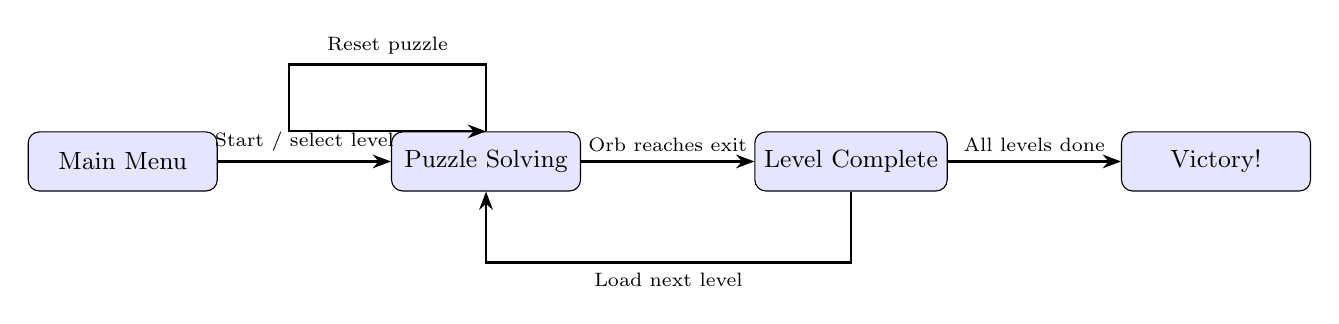
\begin{tikzpicture}[
            node distance=1.0cm and 2.2cm,
            box/.style={draw, rounded corners, minimum width=2.4cm, minimum height=0.75cm,
                        text centered, fill=blue!10, font=\small},
            arr/.style={-{Stealth}, thick},
            lbl/.style={font=\scriptsize, midway}]

            \node[box] (menu)    {Main Menu};
            \node[box, right=of menu]    (puzzle)   {Puzzle Solving};
            \node[box, right=of puzzle]  (complete) {Level Complete};
            \node[box, right=of complete](victory)  {Victory!};

            \draw[arr] (menu)    -- node[lbl, above]{Start / select level} (puzzle);
            \draw[arr] (puzzle)  -- node[lbl, above]{Orb reaches exit}     (complete);
            \draw[arr] (complete)-- node[lbl, above]{All levels done}       (victory);

            % next-level loop back under the nodes
            \draw[arr] (complete.south) -- ++(0,-0.9)
                       -| node[lbl, below, pos=0.25]{Load next level} (puzzle.south);

            % reset self-loop above puzzle node
            \draw[arr] (puzzle.north) -- ++(0,0.85) -- ++(-2.5,0)
                       node[lbl, above, pos=0.5]{Reset puzzle}
                       -- ++(0,-0.85) -- (puzzle.north);
        \end{tikzpicture}
        \end{center}

        \subsubsection{User/Environment --- Obstacles and Props}
        \begin{itemize}[leftmargin=1.5em, itemsep=2pt]
            \item \textbf{Gaps / void.} Any region not covered by a shadow pattern is
                  open void. The Orb falls if it enters a lit gap and respawns at the
                  level start; no objects are moved by the respawn.
            \item \textbf{Static ruins geometry.} Walls, archways, and raised platforms
                  are permanently solid and block both the Orb and shadow propagation.
                  They cannot be moved.
            \item \textbf{Portable lanterns.} Interactable light sources; dragged freely
                  within their boundary. Cast omni-directional shadow behind any object
                  they illuminate.
            \item \textbf{Wall-mounted spotlights.} Interactable light sources; rotated
                  about their fixed mount point. Cast a directed cone of shadow behind
                  objects in their beam.
            \item \textbf{Blocking objects} (pillars, crates). Interactable obstacles;
                  slide along fixed trajectories to reshape the shadows cast by nearby
                  light sources.
            \item \textbf{Exit gate.} A static trigger zone. Completing the level
                  requires the Orb to enter this region while a valid shadow path
                  connects start to exit.
        \end{itemize}

        \subsubsection{User/Character}
        The player never directly controls the Orb's interaction with objects; all
        object manipulation is performed via mouse before or between Orb movements.
        The interaction model is:

        \begin{enumerate}[leftmargin=1.5em, itemsep=2pt]
            \item Player uses the mouse to position light sources and blocking objects,
                  observing how the live shadow pattern changes.
            \item Player uses the keyboard to roll the Orb along the shadow path toward
                  the exit.
            \item If the Orb falls (entered lit void), it respawns at the level start;
                  the player adjusts the configuration and tries again.
            \item When the Orb reaches the exit gate, the level ends and the next
                  level loads automatically.
        \end{enumerate}

        The Reset button is always accessible and returns all objects and the Orb to
        their initial positions for that level.

        \subsubsection{Character/Character}
        There are no NPCs, enemies, or secondary characters. The Orb is the only
        dynamic entity in the scene; all interaction is between the player, the Orb,
        and the environment.

    \subsection{Performance and Scoring}

        \subsubsection{State Variables}
        The following variables are tracked at runtime for each level:

        \begin{itemize}[leftmargin=1.5em, itemsep=2pt]
            \item \textbf{Orb position.} The current world-space position of the Orb.
                  Reset to the level start position on fall or player reset.
            \item \textbf{Lantern position} (one per lantern). The current world-space
                  position of each portable lantern within its movement boundary.
            \item \textbf{Spotlight angle} (one per spotlight). The current rotation
                  angle of each wall-mounted spotlight about its fixed mount point.
            \item \textbf{Blocking object stop index} (one per blocking object). The
                  index of the currently occupied stop position along each object's
                  fixed trajectory.
            \item \textbf{Level completion flag.} Set to true when the Orb enters the
                  exit gate; triggers the level-complete transition.
            \item \textbf{Levels unlocked.} A persistent list of which puzzle levels
                  have been completed, used to populate the level-select screen.
        \end{itemize}

        \subsubsection{Feedback}
        \begin{itemize}[leftmargin=1.5em, itemsep=2pt]
            \item \textbf{Live shadow update.} The shadow boundary redraws continuously
                  as the player drags any light source or blocking object, giving
                  immediate visual confirmation of every change.
            \item \textbf{Object hover highlight.} Interactable objects are visually
                  highlighted when the mouse cursor hovers over them, indicating they
                  can be manipulated.
            \item \textbf{Orb fall.} When the Orb enters a lit gap it plays a brief
                  fall animation and audio cue before respawning at the level start.
                  No objects are moved.
            \item \textbf{Level complete.} Entering the exit gate triggers a short
                  completion animation and a distinct audio cue, followed by an
                  automatic transition to the next level.
            \item \textbf{Interaction sounds.} Distinct sound cues play for lantern
                  drag start/end, spotlight rotation, and blocking object slide.
        \end{itemize}

        \subsubsection{Performance and Progress Metrics}
        Umbra does not record scores, star ratings, move counts, or elapsed time.
        Performance is binary: a level is either complete or not. The only persistent
        metric is the set of levels the player has completed, which unlocks them on
        the level-select screen. There is no leaderboard, no in-game timer display,
        and no penalty for resetting or falling.

% ─── 3. Implementation ───────────────────────────────────────────────────────
\section{Implementation}

    \subsection{Design Assumptions}

        \subsubsection{Hardware}
        Umbra targets standard gaming PC hardware. The primary performance constraint
        is real-time dynamic shadow rendering via Unreal Engine~5's Lumen system.

        \begin{center}
        \begin{tabularx}{\linewidth}{lXX}
            \toprule
            & \textbf{Minimum} & \textbf{Recommended} \\
            \midrule
            OS      & Windows 10 (64-bit)            & Windows 11 (64-bit) \\
            CPU     & Intel Core i5-8400 / AMD Ryzen 5 2600
                    & Intel Core i7-12700 / AMD Ryzen 7 5800X \\
            RAM     & 8 GB                           & 16 GB \\
            GPU     & NVIDIA GTX 1070 / AMD RX 5700  & NVIDIA RTX 3070 / AMD RX 6800 XT \\
            Storage & 4 GB available                 & 8 GB available (SSD) \\
            \bottomrule
        \end{tabularx}
        \end{center}

        \subsubsection{Software}
        \begin{itemize}[leftmargin=1.5em, itemsep=2pt]
            \item \textbf{Game engine.} Unreal Engine~5 (UE5.3 or later), using
                  C++ and Blurprit as wrappers for gameplay logic and Lumen for real-time global
                  illumination and dynamic shadow rendering.
            \item \textbf{Operating system.} Windows 10/11 (64-bit). Development
                  and testing are performed exclusively on Windows.
            \item \textbf{Development IDE.} Visual Studio 2022 (Community or
                  Professional) for any C++ extensions; UE5 editor for Blueprint
                  scripting and level design.
            \item \textbf{Version control.} Git with GitHub for source management;
                  Unreal's \texttt{.gitignore} template applied to exclude derived
                  build artefacts.
            \item \textbf{Asset pipeline.} Blender for 3D modelling and UV unwrapping;
                  Adobe Photoshop / GIMP for texture authoring; Audacity for audio
                  editing.
        \end{itemize}

        \subsubsection{Algorithms and Techniques}
        \begin{itemize}[leftmargin=1.5em, itemsep=2pt]
            \item \textbf{Real-time dynamic shadows (Lumen).} Unreal Engine~5's Lumen
                  global illumination system computes shadow volumes continuously as
                  light source positions and blocking object positions change. No
                  baked lighting is used; all shadows are fully dynamic.
            \item \textbf{Shadow geometry as physical collision.} Shadow-covered
                  regions are mapped to runtime collision volumes. When a light source
                  or blocking object moves, affected collision volumes are updated
                  every frame so the Orb's traversable surface always matches the
                  visible shadow pattern.
            \item \textbf{Lantern drag (boundary-constrained free movement).} A mouse
                  drag event translates the lantern's world position along the
                  camera's view plane. A bounding volume defined per lantern at
                  level-design time clamps the position, preventing the lantern from
                  leaving its valid region.
            \item \textbf{Spotlight rotation (pivot-constrained rotation).} A mouse
                  drag event computes the angle between the spotlight's mount point
                  and the cursor's world-space projection, clamped to a
                  designer-specified angular range.
            \item \textbf{Blocking object trajectory and snap.} Each blocking object
                  follows a pre-defined spline or linear path. When the player
                  interacts with a blocking object, it moves to the nearest valid
                  stop position along its trajectory and snaps into place.
            \item \textbf{Orb physics.} The Orb uses UE5's built-in sphere physics
                  with gravity and rolling friction. Movement is driven by keyboard
                  input applying forces to the physics body; the Orb falls under
                  gravity when it rolls off a shadow edge into lit void.
        \end{itemize}

    \subsection{Storyboards}
    % TODO: Insert concept sketches or storyboard panels showing key game states
    %       (level start, light source drag, blocking object slide, level completion).

    \subsection{Design Logic}

        \subsubsection{Finite State Machines --- Events / States / Effects}

        The game's interaction layer is modelled as a finite state machine with
        seven states. \textbf{Idle} is the default resting state; all others are
        transient and return to Idle (or advance to Level Complete) on their
        terminal event. A \textbf{Reset} event is available in Idle, Orb Moving,
        Lantern Drag, and Spotlight Rotate states; it returns all objects and the
        Orb to their level-start positions and always transitions to Idle.

        \begin{center}
        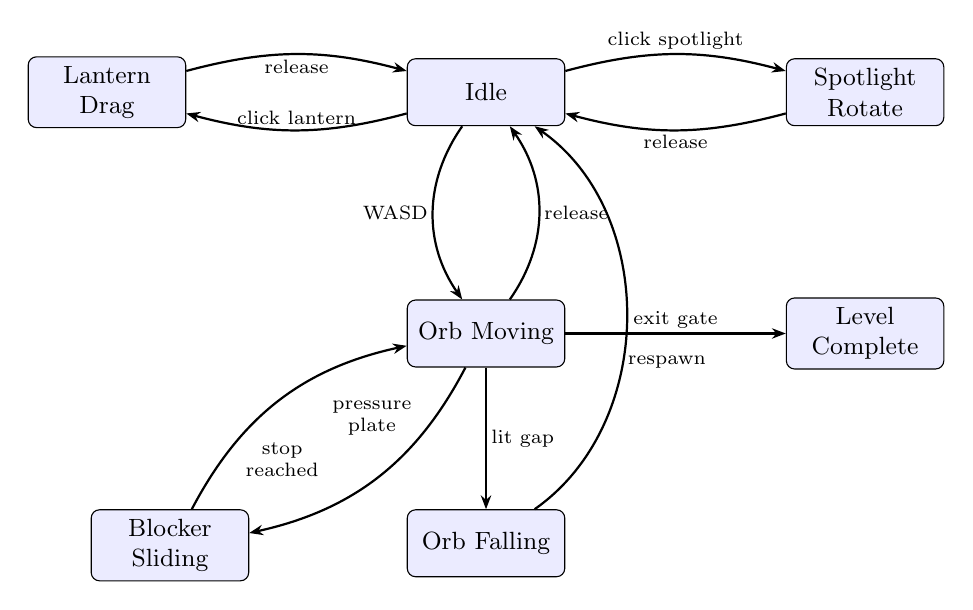
\begin{tikzpicture}[
            node distance=1.5cm and 2.6cm,
            state/.style={draw, rounded corners=3pt, minimum width=2.0cm,
                          minimum height=0.85cm, text centered,
                          fill=blue!8, font=\small, align=center},
            arr/.style={-{Stealth[length=5pt]}, thick},
            lbl/.style={font=\scriptsize, align=center, inner sep=1.5pt}]

            %% ── Nodes ─────────────────────────────────────────────────────
            \node[state]                          (idle)     {Idle};
            \node[state, left=2.8cm  of idle]     (lantern)  {Lantern\\Drag};
            \node[state, right=2.8cm of idle]     (spot)     {Spotlight\\Rotate};
            \node[state, below=2.2cm of idle]     (orbmove)  {Orb Moving};
            \node[state, below left=1.8cm and 2.0cm of orbmove]
                                                  (blocker)  {Blocker\\Sliding};
            \node[state, below=1.8cm of orbmove]  (falling)  {Orb Falling};
            \node[state, right=2.8cm of orbmove]  (complete) {Level\\Complete};

            %% ── Transitions ───────────────────────────────────────────────
            \draw[arr, bend left=15] (idle)    to
                node[lbl, above]{click lantern}  (lantern);
            \draw[arr, bend left=15] (lantern) to
                node[lbl, below]{release}        (idle);

            \draw[arr, bend left=15] (idle) to
                node[lbl, above]{click spotlight} (spot);
            \draw[arr, bend left=15] (spot) to
                node[lbl, below]{release}         (idle);

            \draw[arr, bend right=35] (idle)    to
                node[lbl, left]{WASD}     (orbmove);
            \draw[arr, bend right=35] (orbmove) to
                node[lbl, right]{release} (idle);

            \draw[arr, bend left=25] (orbmove) to
                node[lbl, above left, pos=0.3]{pressure\\plate} (blocker);
            \draw[arr, bend left=25] (blocker) to
                node[lbl, below right, pos=0.3]{stop\\reached}  (orbmove);

            \draw[arr] (orbmove) to
                node[lbl, right]{lit gap}    (falling);
            \draw[arr, bend right=55] (falling) to
                node[lbl, right, pos=0.4]{respawn} (idle);

            \draw[arr] (orbmove) to
                node[lbl, above]{exit gate} (complete);

        \end{tikzpicture}
        \end{center}

        \medskip\noindent\textbf{State descriptions:}
        \begin{itemize}[leftmargin=1.5em, itemsep=2pt]
            \item \textbf{Idle.} Default state. No input is being processed.
                  The player may hover over interactable objects, press WASD,
                  click a light source, or press Reset.
            \item \textbf{Lantern Drag.} Left mouse button is held on a
                  portable lantern. The lantern follows the cursor world-space
                  projection each frame, clamped to its movement boundary.
                  Shadow geometry updates continuously. Released mouse button
                  returns to Idle.
            \item \textbf{Spotlight Rotate.} Left mouse button is held on a
                  wall-mounted spotlight. The spotlight angle is driven by the
                  cursor's angular offset from the mount point each frame,
                  clamped to the designer-specified range. Shadow geometry
                  updates continuously. Released mouse button returns to Idle.
            \item \textbf{Orb Moving.} WASD is held; input forces are applied
                  to the Orb's physics body each frame. Stepping on a pressure
                  plate transitions to Blocker Sliding (then back). Entering
                  a lit gap transitions to Orb Falling. Reaching the exit gate
                  transitions to Level Complete.
            \item \textbf{Blocker Sliding.} A blocking object is animating
                  along its trajectory toward the next stop position. Player
                  input is suspended. When the object snaps to the stop, the
                  machine returns to Orb Moving.
            \item \textbf{Orb Falling.} The Orb has entered lit void. A brief
                  fall animation and audio cue play. All objects remain where
                  the player left them. On animation end the Orb respawns at
                  the level start and the machine returns to Idle.
            \item \textbf{Level Complete.} The Orb has entered the exit gate.
                  A completion animation and audio cue play, then the next
                  level loads (or the Victory screen if all levels are done).
        \end{itemize}

        \subsubsection{User Solution / Actions}

        The following walkthrough traces a complete solution to the tutorial
        level (\textbf{The Antechamber}) and maps each player action to the
        corresponding FSM transitions.

        \begin{enumerate}[leftmargin=1.5em, itemsep=4pt]

            \item \textbf{Level loads --- Idle.}
                  The Orb sits at the start position. A portable lantern rests
                  near the centre of the platform, casting light away from a
                  gap that blocks the path to the exit. A blocking pillar
                  stands to the side of the gap, and a pressure plate is
                  visible beyond the first gap.

            \item \textbf{Drag the lantern to bridge the first gap
                  (Idle $\to$ Lantern Drag $\to$ Idle).}
                  The player clicks and holds the lantern, then drags it
                  toward the near edge of the gap. As the lantern moves, its
                  shadow sweeps across the void, and the gap region gradually
                  becomes physically solid. When the shadow fully spans the
                  gap the player releases the mouse. The machine returns to
                  Idle with the gap bridged by shadow.

            \item \textbf{Roll the Orb across the shadow bridge
                  (Idle $\to$ Orb Moving $\to$ Idle).}
                  The player presses WASD to roll the Orb forward along the
                  shadow-covered path. The Orb crosses the gap without falling
                  because the shadow beneath it is solid. The player releases
                  WASD after reaching the far platform; the machine returns to
                  Idle.

            \item \textbf{Trigger the pressure plate to slide the pillar
                  (Idle $\to$ Orb Moving $\to$ Blocker Sliding $\to$
                  Orb Moving $\to$ Idle).}
                  A second gap separates the far platform from the exit. The
                  blocking pillar, if repositioned, would cast a shadow that
                  spans it. The player presses WASD to roll the Orb onto the
                  pressure plate marked on the floor. The Orb Moving state
                  detects the pressure-plate overlap and transitions to Blocker
                  Sliding: the pillar animates along its fixed trajectory to
                  its second stop position, now blocking the light source from
                  the correct angle. The shadow extends across the second gap.
                  Once the pillar snaps to the stop the machine returns to Orb
                  Moving. The player releases WASD; the machine returns to
                  Idle.

            \item \textbf{Roll the Orb to the exit gate
                  (Idle $\to$ Orb Moving $\to$ Level Complete).}
                  The player presses WASD to roll the Orb along the newly
                  formed shadow path across the second gap and into the exit
                  gate. The Orb Moving state detects the exit-gate overlap and
                  transitions to Level Complete. The completion animation plays
                  and the next level loads.

        \end{enumerate}

    \subsection{Software Versions}

        \subsubsection{Alpha Version}
        \textit{Due: Wed.\ Mar.\ 18.} The Alpha is a vertical slice demonstrating
        all core mechanics in a single fully playable level.

        \begin{itemize}[leftmargin=1.5em, itemsep=2pt]
            \item \textbf{Core shadow mechanic.} Real-time dynamic shadows; shadow-covered regions are mapped to runtime
                  collision volumes so the Orb can traverse them.
            \item \textbf{Lantern drag.} One portable lantern freely draggable
                  within its boundary constraint; shadow updates continuously.
            \item \textbf{Blocking objects and pressure plates.} One or two
                  blocking objects that slide to designer-specified stop
                  positions when the Orb steps on the corresponding pressure
                  plate.
            \item \textbf{Orb physics.} Keyboard-driven sphere with UE5
                  physics: gravity, rolling friction, and respawn on fall.
            \item \textbf{One playable level.} \textit{Level 1 --- The
                  Collapsed Bridge}: a single self-contained puzzle using the
                  lantern and two blocking pillars to span a central chasm.
            \item \textbf{Minimal UI.} Level name display and a Reset button
                  (returns all objects and the Orb to start positions).
            \item \textbf{Placeholder art and audio.} Untextured geometry and
                  placeholder sound cues sufficient for playtesting.
        \end{itemize}

        \subsubsection{Beta Version}
        \textit{Due: Wed.\ Mar.\ 25.} The Beta expands the Alpha to a
        complete multi-level experience with polished content and secondary
        mechanics.

        \begin{itemize}[leftmargin=1.5em, itemsep=2pt]
            \item \textbf{Spotlight rotation.} Wall-mounted spotlights
                  freely rotatable within their angular range; directed-cone
                  shadow updates continuously.
            \item \textbf{All puzzle levels.} \textit{Level 2 --- The Torch
                  Hall} (spotlights + blocking objects) and \textit{Level 3
                  --- The Inner Sanctum} (combined mechanics) added and
                  playable end-to-end.
            \item \textbf{Tutorial level.} \textit{The Antechamber} included
                  with on-screen prompts (see \S3.4.3).
            \item \textbf{Level-select screen.} Main menu listing all four
                  spaces; completed levels are marked unlocked.
            \item \textbf{Victory screen.} Displayed after completing all
                  three puzzle levels.
            \item \textbf{Polished art.} Textured Roman-ruin geometry,
                  particle effects on light sources, and atmospheric skybox.
            \item \textbf{Polished audio.} Ambient music track, distinct
                  sound cues for lantern drag, spotlight rotation, blocker
                  slide, Orb fall, and level completion.
            \item \textbf{Hover highlights.} Interactable objects highlight
                  on mouse-over to communicate affordance clearly.
            \item \textbf{Bug fixes and playtest feedback.} Issues identified
                  in the Alpha playtest resolved; puzzle difficulty tuned.
        \end{itemize}

        \subsubsection{Tutorials}
        The tutorial level (\textbf{The Antechamber}) is a short, guided
        introduction that teaches all three interaction mechanics in sequence
        with no dead ends and no prior knowledge required.

        \begin{enumerate}[leftmargin=1.5em, itemsep=4pt]
            \item \textbf{Shadow mechanic introduction.} A single gap
                  separates the Orb from a small platform. A lantern is
                  already positioned so its shadow almost spans the gap.
                  An on-screen prompt reads: \textit{``Drag the lantern to
                  cast a shadow bridge.''}  The player adjusts the lantern;
                  the shadow snaps across the gap.  A second prompt reads:
                  \textit{``Walk across the bridge.''} 

            \item \textbf{Pressure-plate and blocking-object introduction.}
                  The Orb arrives at a second gap. A pressure plate is
                  visible on the current platform, and a blocking pillar
                  stands nearby. An on-screen prompt reads: \textit{``Step
                  on the pressure plate to move the pillar.''}  The Orb
                  rolls onto the plate; the pillar slides to its second stop,
                  extending the lantern's shadow across the second gap.  The
                  player rolls the Orb across to complete the level.

            \item \textbf{Respawn demonstration (optional).}  If the player
                  rolls the Orb into a void before completing either step,
                  the fall animation plays and the Orb respawns at the level
                  start with all objects in their current positions.  No
                  explicit prompt is shown; the mechanic is self-evident.
        \end{enumerate}

        On-screen prompts appear as brief text overlays anchored to the
        relevant object and disappear automatically once the player performs
        the indicated action. No prompts appear in the three main puzzle
        levels; the tutorial is the only guided section of the game.

% ─── 4. Work Plan ────────────────────────────────────────────────────────────
\section{Work Plan}

    \subsection{Tasks}

    \noindent CC = Cecilia Chen \quad JP = Jacky Park \quad YT = Yiding Tian

    \medskip
    \begin{center}
    \begin{tabular}{p{0.7cm} p{7.2cm} c c}
    \hline
     & \textbf{Task} & \textbf{Time (days)} & \textbf{Member} \\
    \hline
    1   & Set up base project (UE5, Git, asset folders)      & 3  & All    \\
    \hline
    2   & \textbf{Shadow and Light System}                   &    &        \\
    \hline
    2.1 & Lumen real-time shadow configuration               & 5  & CC     \\
    2.2 & Shadow-to-collision volume mapping                 & 7  & CC, JP \\
    2.3 & Lantern boundary constraint system                 & 3  & JP     \\
    2.4 & Spotlight angular constraint system                & 3  & JP     \\
    \hline
    3   & \textbf{Player Interaction}                        &    &        \\
    \hline
    3.1 & Lantern drag (mouse-to-world, boundary clamp)      & 4  & JP     \\
    3.2 & Spotlight rotation (cursor angle, range clamp)     & 3  & JP     \\
    3.3 & Pressure plate trigger                             & 2  & JP     \\
    3.4 & Blocking object trajectory and snap                & 4  & JP     \\
    3.5 & Object hover highlight                             & 2  & JP     \\
    \hline
    4   & \textbf{Orb Character}                             &    &        \\
    \hline
    4.1 & Sphere physics setup                               & 3  & CC     \\
    4.2 & WASD keyboard input                                & 2  & CC     \\
    4.3 & Fall detection and respawn                         & 2  & CC     \\
    \hline
    5   & \textbf{Level Design}                              &    &        \\
    \hline
    5.1 & Tutorial --- The Antechamber                       & 4  & All     \\
    5.2 & Level 1 --- The Collapsed Bridge                   & 5  & All     \\
    5.3 & Level 2 --- The Torch Hall                         & 5  & All     \\
    5.4 & Level 3 --- The Inner Sanctum                      & 7  & All     \\
    \hline
    6   & \textbf{UI and HUD}                                &    &        \\
    \hline
    6.1 & Main menu and level-select screen                  & 4  & YT     \\
    6.2 & In-game HUD and Reset button                       & 2  & YT     \\
    6.3 & Level-complete and Victory screens                 & 2  & YT     \\
    6.4 & Tutorial on-screen prompts                         & 2  & YT     \\
    \hline
    7   & \textbf{Art and Assets}                            &    &        \\
    \hline
    7.1 & Orb model and texture                              & 3  & CC     \\
    7.2 & Environment geometry (platforms, ruins)            & 7  & YT     \\
    7.3 & Light source models (lantern, spotlight)           & 3  & YT     \\
    7.4 & Blocking object models (pillar, crate)             & 3  & YT     \\
    7.5 & Particle effects and skybox                        & 3  & YT     \\
    \hline
    8   & \textbf{Audio}                                     &    &        \\
    \hline
    8.1 & Ambient background music                           & 3  & YT     \\
    8.2 & Sound effects                                      & 3  & YT     \\
    \hline
    9   & Testing                                            & 7  & All    \\
    \hline
    10  & Polishing and extra features                       &    & All    \\
    \hline
    \end{tabular}
    \end{center}

    \subsection{Milestones}

        \subsubsection{Minor Milestones}

        \begin{center}
        \begin{tabular}{p{2.4cm} p{9.5cm}}
        \hline
        \textbf{Date} & \textbf{Milestone} \\
        \hline
        Wed.\ Mar.\ 4  & UE5 project initialized; Git repo set up; all members able to build and run \\
        Sat.\ Mar.\ 7  & Real-time Lumen shadows working: moving a light source visibly reshapes the cast shadow \\
        Tue.\ Mar.\ 10 & Shadow-to-collision mapping working: Orb can traverse shadow-covered regions and falls into lit void \\
        Thu.\ Mar.\ 12 & Orb physics complete: WASD movement, gravity, rolling friction, fall detection, and respawn \\
        Sat.\ Mar.\ 14 & Lantern drag with boundary constraint working; pressure plate trigger and blocker snap working \\
        Mon.\ Mar.\ 16 & Level 1 full loop playable: lantern, two blockers, exit gate, Reset button \\
        Fri.\ Mar.\ 20 & Spotlight rotation working; all four level layouts blocked out \\
        Mon.\ Mar.\ 23 & Tutorial level with on-screen prompts complete; level-select screen and all UI screens implemented \\
        Thu.\ Mar.\ 26 & Full art pass complete: all meshes textured, particle effects and skybox in place \\
        Sat.\ Mar.\ 28 & Audio complete: ambient music and all sound effects integrated \\
        Sun.\ Mar.\ 29 & Final bug fixes, puzzle tuning, and performance pass complete \\
        \hline
        \end{tabular}
        \end{center}

        \subsubsection{Major Milestones}

        \begin{center}
        \begin{tabular}{p{2.4cm} p{9.5cm}}
        \hline
        \textbf{Date} & \textbf{Milestone} \\
        \hline
        Mon.\ Mar.\ 2  & Game Design Document submitted \\
        Wed.\ Mar.\ 18 & Alpha Version / Playtest: one fully playable level with core shadow mechanic \\
        Wed.\ Mar.\ 25 & Beta Version / Playtest: all four levels, polished art and audio, complete UI \\
        Mon.\ Mar.\ 30 & Final Version / Demo: release build packaged and submitted \\
        Wed.\ Apr.\ 1  & Game Trailer and Gameplay Videos submitted \\
        \hline
        \end{tabular}
        \end{center}

    \newpage
    \subsection{Development Schedule}

    \begin{figure}[h]
        \centering
        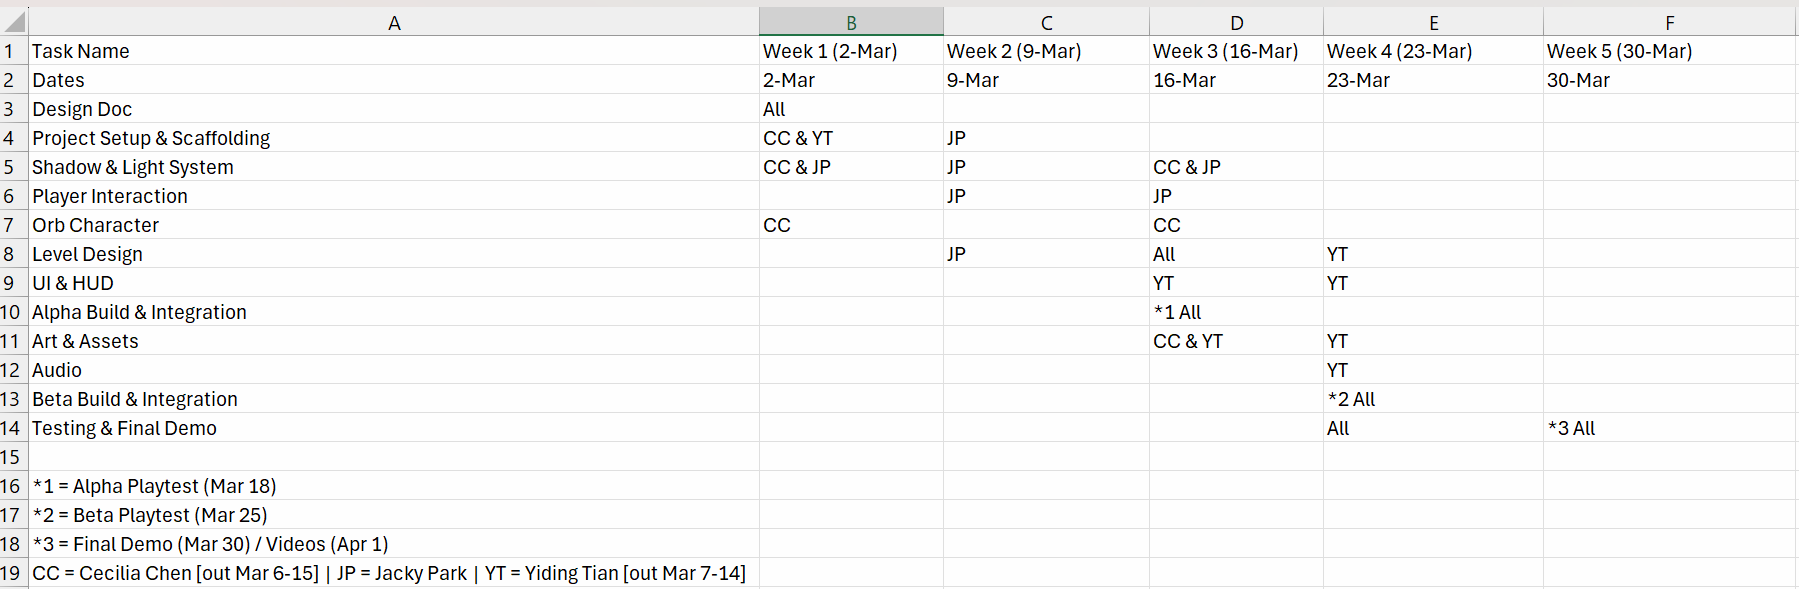
\includegraphics[width=\linewidth]{img/Gantt.png}
    \end{figure}

\end{document}
